% !TEX root =../main.tex

\chapter{Auswahl an Konzepten Festlegen}


\section{Voraussetzung bei der Entwicklung}


\subsection{Viskosität zwischen Nutzer und die Webseite verstärken}

Laut Nielsen, ein Marktforschungsunternehmen, Instant Messaging, Kommentar, Bloggen, Teilen und "Lob" machen jetzt 22\% der gesamten monatlichen Online-Zeit. Nielsens am Dienstag veröffentlichte Statistiken zeigten, dass Menschen alle 4,5 Minuten in sozialen Netzwerken oder Blogs eine Minute ihrer Online-Zeit verbringen. Internetnutzer verbringen jeden Monat 110 Milliarden Minuten in sozialen Netzwerken und Blogs. Die Umfrage sagte dies das erste Mal ist ein soziales Netzwerk oder ein Blog „ist drei Viertel der Online-Nutzer auf der Welt zugreifen können.“ Das ist eine Steigerung von 24\% gegenüber dem gleichen Zeitraum des Vorjahres. Die beliebtesten Social-Networking-Marken sind Facebook und YouTube. Online-Nutzer haben im vergangenen Monat 13 Milliarden Videos auf YouTube gesehen. Facebook sagte auch, dass seine Nutzer 2 Milliarden Videos pro Monat sehen.

Laut Nielsens Studie hat Facebook in den globalen Online-Stunden das Rampenlicht übernommen. Fast 500 Millionen Nutzer verbringen jeden Monat sechs Stunden damit.
Was die Netzabdeckung betrifft, übernimmt Google die Führung. Laut Nielsen-Statistiken besuchen 82\% der Internetnutzer weltweit jeden Monat die Website, und die durchschnittliche Such- und Suchzeit beträgt 1 Minute und 20 Sekunden.(Nielsen-Studie: Facebook und Google haben erfolgreichste Apps   Jonas Wagner)

d.h. die Länge der Online -Zeit bleiben Nutzer auf eine Webseite, ist ein Zeichen, ob die Webseit beliebt ist und die  Viskosität stark ist.

Ein Ziel ist, wie kann man die Nutzer mehrere Zeit auf die Webseite bei der Entwurf bleiben lassen.
Mehr interessante Funktionen und Verstaltung?


\subsection{die mehrere Produkte verkaufte online Shops sind beliebt}

Nach der Statistik von Alexa in Abbildung \vref{fig:alexa}, top 10 online Shops mit dem höchsten Umsatz in der Welt sind Amazon, netflix, ebay, walmart, etsy, Store.steampowered.com, ikea, usw. sie haben eine Gesamtheit, die vielfalte  Produkte vorhanden.

\begin{figure}
	\centering
	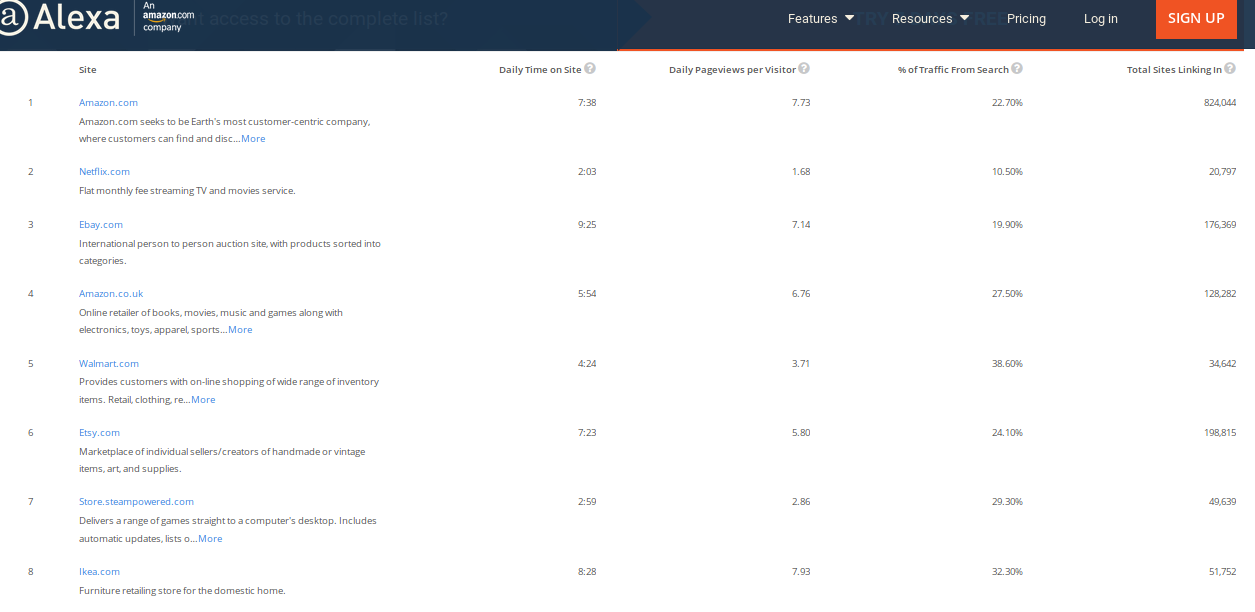
\includegraphics[width=1\textwidth]{bilder/alexa.png}
	\caption{Alexa}
	\label{fig:alexa}
\end{figure}


\section{Freundesliste organisation}

man Listen verwenden, um  Freunde organisieren. Mit einer Liste kann man die Meldungen in seinem News Feed filtern oder Aktualisierungen mit bestimmten Personen teilen, z. B. mit deinen Arbeitskollegen oder Freunden, die in deiner Nähe wohnen. man kann jederzeit hinzufügen order entfernen .  Quelle: Facebook. https://de-de.facebook.com/help/204604196335128

\textbf{Enge Freunde:} Freunde, mit denen man möglicherweise exklusiv teilen möchte.

\textbf{Bekannte:} Personen, mit denen man eventuell weniger teilen möchtest.

\textbf{Eingeschränkt:} Diese Liste ist für Personen, die man als Freunde hinzugefügt hat, mit denen man aber nichts teilen möchte, z. B. dein Chef.

Man kann außerdem selbst definierte Liste erstellen,  um selbst Freunde in Gruppen zusammenzufassen. Du legst fest, wer zu dieser Liste hinzugefügt wird und welche Privatsphäre-Einstellungen (gegebenenfalls) gelten. Beachte, dass deine Freunde nicht benachrichtigt werden, wenn du sie zu benutzerdefinierten Listen hinzufügst.


\section{real Time Kommunikation mit andere Nutzer , Verkäufer und Customer Service der Plattform}

Es gibt ein Nachteil von Amazon, schwer mit Verkäufer  und Nach Kauf-Service verbinden, damit Waren oder Logik – Probleme entstehen.

Wenn die real Time Kommunikation ausführt , kann man schnell die Probleme löschen und Zeit sparen, gut Kauf- Experiment haben.


\section{Wie kann man machen, wenn die nötige Freund offline ist.}

Gleichzeit eine URL- Nachricht bei Email und SMS senden, die mit Produktinformation inklusieren. Freunde oder Bekannte müssen nicht mehr noch einmal anmelden, direkt die URL antippen und bereits loggen, dann Vorschlag oder Entscheidung zu machen helfen.


\section{Nach dem Handel, die Erfahrung und Bewertung mitteilen und Produkt Zeigen}


\section{pay by others}

wenn Kind brauche finanzielle Hilfe von Eltern, die Eltern können auch auf die Webseite einloggen und entscheiden, ob sie für Kinder ‘s  Kauf  bezahlen wollen.


\section{zusätzliche Service}


\subsection{weitere Entwicklung basis auf ebay kleinzeigen}

von ebay kleinzeigen zu online Flohmarkt.

Gebrauchte Produkte zeigen auf die Webseite, nicht mehr nach der einzelnen Attribute zu klassieren, sondern nach die Gruppe der Familie zusammen hochladen. Sowie man geht zum Flohmarkt, die gebrauchte Dinge steht nicht nach die Attribute, z.B. alle Verkäufer im Markt stehen nicht  alle Spielzeuge zusammen zu verkaufen, sondern alleine verkaufen unterschiedlichen Produkte.


\subsection{Communities  für die Nutzer ertstellen, um die Nachricht zu veröffentlichen und Erfahrung auszutauschen}

\begin{itemize}
\item Kooperation existiert vor allem in Computerspielen
\item Darstellung und Interaktion mit WebShop wird denen von Computerspielen nachempfunden
\item 3D Darstellung und Steuerung wie in Computerspielen
\end{itemize}